% !TeX program = xelatex
% Báo cáo độc lập; khi tích hợp báo cáo tổng chỉ cần \input hai tệp trong chapters/.
\documentclass[12pt,a4paper,oneside]{report}
\input{../../Latex/LATEX_TASK2_(2.1-2.7+4.1-4.2)/config/preamble}

\usepackage{listings}
\lstdefinestyle{pythonreport}{
  language=Python,
  basicstyle=\ttfamily\scriptsize,
  keywordstyle=\color{mtdark}\bfseries,
  commentstyle=\color{gray},
  stringstyle=\color{teal!70!black},
  numbers=left,
  numberstyle=\tiny\color{gray},
  stepnumber=1,
  numbersep=7pt,
  frame=single,
  rulecolor=\color{gray!50},
  breaklines=true,
  breakatwhitespace=false,
  showstringspaces=false,
  columns=fullflexible,
  keepspaces=true,
  xleftmargin=1.2em,
  framexleftmargin=1em
}
\lstset{style=pythonreport}
\renewcommand{\lstlistingname}{Đoạn mã}
\renewcommand{\lstlistlistingname}{Danh mục đoạn mã}
\setlength{\emergencystretch}{2em}
\graphicspath{{../figures/}}

\begin{document}
\begin{titlepage}
  \centering
  {\large ĐẠI HỌC QUỐC GIA THÀNH PHỐ HỒ CHÍ MINH\par}
  {\large TRƯỜNG ĐẠI HỌC BÁCH KHOA\par}
  \vspace{2.4cm}
  {\Large\bfseries BÁO CÁO BÀI TẬP LỚN\par}
  \vspace{0.4cm}
  {\Large\bfseries XÁC SUẤT VÀ THỐNG KÊ (MT2013)\par}
  \vspace{1.5cm}
  {\LARGE\bfseries KIỂM ĐỊNH GIẢ THUYẾT HAI MẪU ĐỘC LẬP TRÊN BỘ DỮ LIỆU NSL-KDD\par}
  \vfill
  {\large Phần bổ sung cho Chương 3 và Chương 4\par}
  \vspace{1cm}
  {\large Thành phố Hồ Chí Minh, năm 2026\par}
\end{titlepage}

\pagenumbering{roman}
\tableofcontents
\clearpage
\listoffigures
\clearpage
\listoftables
\clearpage
\pagenumbering{arabic}

\setcounter{chapter}{2}
\chapter{Phương pháp Xác suất và Thống kê}
\setcounter{section}{5}
% Tệp thành phần: không chứa preamble hoặc môi trường document.
\section{Kiểm định giả thuyết hai mẫu độc lập}
\label{sec:two-sample-method}

Nhãn nhị phân của nghiên cứu gộp DoS, Probe, R2L và U2R thành nhóm Attack, trong
khi giữ Normal là nhóm đối chứng. Vì vậy, kiểm định hai mẫu được dùng để đánh giá
liệu trung bình của một đặc trưng lưu lượng có khác nhau giữa hai nhãn này hay không.
Phép kiểm định bổ sung cho ANOVA năm nhóm: ANOVA bảo toàn sự không đồng nhất giữa
bốn họ tấn công, còn kiểm định hai mẫu trả lời tương phản trực tiếp Normal--Attack.
Nó cũng khác Pearson, vì Pearson đo liên hệ tuyến tính giữa hai biến định lượng chứ
không trực tiếp kiểm định chênh lệch trung bình theo nhãn. Thống kê mô tả cho biết vị
trí và độ phân tán quan sát được, nhưng chưa định lượng độ bất định của chênh lệch.

Mục tiêu của phân tích là cung cấp bằng chứng suy diễn và kích thước khác biệt cho
những đặc trưng có ý nghĩa hành vi mạng. Kết quả không được xem là thước đo trực tiếp
của năng lực dự đoán và không chứng minh nhãn tấn công gây ra giá trị đặc trưng.

\subsection{Mục tiêu và câu hỏi nghiên cứu}
\label{subsec:two-sample-rq}

Ba câu hỏi được xác định trước khi xem kết quả kiểm định:
\begin{enumerate}[label=\textbf{RQ\arabic*:},leftmargin=1.7cm]
  \item Tỷ lệ lỗi SYN trung bình của các kết nối đến cùng dịch vụ
  (\path{srv_serror_rate}) có khác nhau giữa Normal và Attack hay không?
  \item Tỷ lệ lỗi REJ trung bình của các kết nối đến cùng dịch vụ
  (\path{srv_rerror_rate}) có khác nhau giữa hai nhóm hay không?
  \item Số kết nối gần đây trung bình (\texttt{count}) có khác nhau giữa hai nhóm
  hay không?
\end{enumerate}

Hai biến đầu là tỷ lệ trong miền $[0,1]$, lần lượt phản ánh lỗi SYN và lỗi REJ trong
tập kết nối đến cùng dịch vụ. \texttt{count} đếm số kết nối đến cùng máy đích trong
cửa sổ hai giây, nên là biến đếm rời rạc. Ba biến được chọn vì đại diện cho lỗi thiết
lập kết nối, lỗi từ chối và cường độ kết nối; chúng không phải một bước sàng lọc toàn
bộ 41 đặc trưng của NSL-KDD.

\subsection{Cơ sở lý thuyết của kiểm định hai mẫu độc lập}
\label{subsec:two-sample-theory}

Gọi $g\in\{N,A\}$ lần lượt là Normal và Attack; $n_g$, $\bar{x}_g$, $s_g^2$ và
$\mu_g$ là cỡ mẫu, trung bình mẫu, phương sai mẫu và trung bình tổng thể. Các thống
kê trong từng nhóm được xác định bởi
\begin{equation}
  \bar{x}_g=\frac{1}{n_g}\sum_{i=1}^{n_g}x_{gi},
  \label{eq:two-sample-mean}
\end{equation}
\begin{equation}
  s_g^2=\frac{1}{n_g-1}\sum_{i=1}^{n_g}(x_{gi}-\bar{x}_g)^2.
  \label{eq:two-sample-variance}
\end{equation}
Ước lượng điểm của chênh lệch trung bình là
\begin{equation}
  \widehat{\Delta}=\bar{x}_N-\bar{x}_A,
  \label{eq:two-sample-difference}
\end{equation}
trong đó dấu âm nghĩa là trung bình Attack lớn hơn trung bình Normal. Do phương sai
hai nhóm không được giả định bằng nhau, sai số chuẩn Welch là
\begin{equation}
  SE(\widehat{\Delta})=
  \sqrt{\frac{s_N^2}{n_N}+\frac{s_A^2}{n_A}}.
  \label{eq:welch-se}
\end{equation}
Thống kê kiểm định và bậc tự do Welch--Satterthwaite lần lượt là
\begin{equation}
  t=\frac{\bar{x}_N-\bar{x}_A}
  {\sqrt{\frac{s_N^2}{n_N}+\frac{s_A^2}{n_A}}},
  \label{eq:welch-t}
\end{equation}
\begin{equation}
  \nu=
  \frac{\left(\frac{s_N^2}{n_N}+\frac{s_A^2}{n_A}\right)^2}
  {\frac{\left(\frac{s_N^2}{n_N}\right)^2}{n_N-1}
  +\frac{\left(\frac{s_A^2}{n_A}\right)^2}{n_A-1}}.
  \label{eq:welch-df}
\end{equation}
Khoảng tin cậy hai phía cho chênh lệch trung bình được tính nhất quán với kiểm định:
\begin{equation}
  CI_{95\%}(\mu_N-\mu_A)=
  \widehat{\Delta}\pm t_{0.975,\nu}SE(\widehat{\Delta}).
  \label{eq:welch-ci}
\end{equation}
Các khoảng ở Công thức~\eqref{eq:welch-ci} là khoảng riêng lẻ cho từng RQ, không tự
động bảo đảm độ bao phủ đồng thời 95\% cho cả ba câu hỏi.

Ngoài chênh lệch trên đơn vị gốc, nghiên cứu báo cáo Cohen $d$ và Hedges $g$ theo quy
ước độ lệch chuẩn gộp. Với $s_p$ là độ lệch chuẩn gộp,
\begin{equation}
  d=\frac{\bar{x}_N-\bar{x}_A}{s_p},\qquad
  g=\left(1-\frac{3}{4(n_N+n_A)-9}\right)d.
  \label{eq:hedges-g}
\end{equation}
Do phương sai thực tế khác nhau, $g$ được dùng như chỉ số chuẩn hóa mô tả; chênh lệch
và khoảng tin cậy trên thang gốc vẫn là kết quả ưu tiên để diễn giải.

\subsection{Xây dựng giả thuyết thống kê}
\label{subsec:two-sample-hypotheses}

Với từng RQ, giả thuyết hai phía là
\begin{equation}
  H_0:\mu_N=\mu_A,
  \qquad
  H_1:\mu_N\ne\mu_A.
  \label{eq:two-sample-hypotheses}
\end{equation}
Kiểm định hai phía được chọn vì nghiên cứu không áp đặt trước chiều khác biệt. Ở mức
$\alpha=0{,}05$, $H_0$ bị bác bỏ khi p-value đã hiệu chỉnh nhỏ hơn $\alpha$. Không
bác bỏ $H_0$ chỉ có nghĩa dữ liệu chưa cung cấp đủ bằng chứng cho khác biệt, không phải
chứng minh hai trung bình bằng nhau. Vì có ba kiểm định chính, phương pháp Holm được
dùng để kiểm soát sai lầm loại I theo họ giả thuyết; p-value thô và p-value Holm được
báo cáo riêng.

\subsection{Giả định và chẩn đoán}
\label{subsec:two-sample-assumptions}

Thứ nhất, hai mẫu phải độc lập giữa và trong nhóm. Nhãn Normal và Attack không giao
nhau, nhưng NSL-KDD không cung cấp định danh phiên hoặc máy nguồn đủ để kiểm tra các
kết nối có thuộc cùng một hoạt động hay không. Welch không khắc phục được phụ thuộc
tiềm ẩn này, vì vậy suy luận được xem là khám phá có điều kiện trên cấu trúc dữ liệu.

Thứ hai, phân phối trung bình mẫu cần được xấp xỉ hợp lý. Histogram/ECDF mô tả toàn bộ
phân bố; boxplot cho thấy trung vị, IQR và ngoại lệ; Q--Q plot đối chiếu các phân vị
quan sát với phân vị chuẩn. Shapiro--Wilk trên tối đa 5.000 quan sát mỗi nhóm chỉ là
chẩn đoán bổ sung, không phải quy tắc lựa chọn duy nhất. Cỡ mẫu lớn làm trung bình mẫu
ổn định hơn, nhưng không biến các quan sát gốc thành phân phối chuẩn.

Thứ ba, Brown--Forsythe (Levene với tâm là trung vị) được dùng để đánh giá chênh lệch
phương sai. Welch không yêu cầu phương sai bằng nhau, song vẫn nhạy với phụ thuộc và
các phân bố quá dị biệt. Hai biến tỷ lệ bị chặn và có khối lượng tại 0 hoặc 1;
\texttt{count} là biến đếm lệch phải và có ngoại lệ. Do đó, Mann--Whitney U và
Yuen--Welch với trung bình cắt ngọn 20\% được dùng như phân tích độ nhạy. Chúng không
kiểm định đúng cùng tham số với trung bình gốc nên không thay thế kết quả chính.

\subsection{Quy trình thực hiện}
\label{subsec:two-sample-procedure}

Dữ liệu đầu vào là KDDTrain+ đã làm sạch, còn KDDTest+ được giữ riêng cho đánh giá mô
hình. Nhóm kiểm tra miền giá trị, kiểu dữ liệu, thiếu, NaN và vô hạn; sau đó xác nhận
\texttt{label\_binary}=0 tương ứng Normal và mọi nhãn DoS, Probe, R2L, U2R tương ứng
Attack. Không sử dụng SMOTE, StandardScaler hoặc bản ghi tổng hợp và không loại ngoại
lệ để làm thay đổi p-value.

Trên mỗi đặc trưng, quy trình lần lượt: (i) tính thống kê mô tả và CI trung bình từng
nhóm; (ii) khảo sát boxplot, ECDF, Q--Q plot, skewness, khối lượng tại biên và tỷ số
phương sai; (iii) chạy Welch hai phía trên toàn bộ quan sát hợp lệ; (iv) tính CI của
chênh lệch và Hedges $g$; (v) hiệu chỉnh Holm ba p-value chính; (vi) đối chiếu
Mann--Whitney U và Yuen--Welch; (vii) diễn giải theo hướng dữ liệu, không theo quan hệ
nhân quả. Chỉ ECDF và Q--Q plot được lấy mẫu cố định lần lượt tối đa 5.000 và 1.000
quan sát/nhóm với \texttt{random\_state}=18015; kiểm định dùng toàn bộ dữ liệu.

\subsection{Công cụ triển khai}
\label{subsec:two-sample-tools}

Pandas và NumPy được dùng để đọc, kiểm tra và tổng hợp dữ liệu; SciPy thực hiện các
phân phối, Brown--Forsythe, Mann--Whitney và Yuen--Welch; Statsmodels hiệu chỉnh Holm.
Matplotlib và Seaborn tạo hình PNG 300 DPI và SVG. Mã nguồn, kiểm thử và bảng kết quả
được lưu trong thư mục \texttt{two\_sample\_testing}; phần kết quả được trình bày tại
Mục~\ref{sec:two-sample-results}.



\setcounter{chapter}{3}
\chapter{Kết quả và thảo luận}
\setcounter{section}{5}
% Tệp thành phần: số liệu đối chiếu với CSV trong two_sample_testing/results.
\section{Kết quả kiểm định hai mẫu độc lập}
\label{sec:two-sample-results}

Phân tích sử dụng toàn bộ 125.973 bản ghi KDDTrain+ hợp lệ, gồm 67.343 Normal và
58.630 Attack. Ba đặc trưng được kiểm định trên thang gốc bằng Welch hai phía tại
$\alpha=0{,}05$; ba p-value chính được hiệu chỉnh Holm. Không có bản ghi nào bị loại
do thiếu, NaN, vô hạn hoặc sai miền. Các p-value bị underflow số học được trình bày
là $p<10^{-300}$, không viết $p=0$.

\subsection{Thống kê mô tả}
\label{subsec:two-sample-descriptive}

Bảng~\ref{tab:two-sample-descriptive} cho thấy hai nhóm chỉ mất cân bằng nhẹ về cỡ
mẫu (tỷ số 1,149), nhưng vị trí và độ phân tán khác nhau rõ. Đặc biệt, phương sai của
Attack lớn hơn Normal ở cả ba biến.

\begin{table}[H]
\centering
\caption{Thống kê mô tả ba đặc trưng theo nhãn trên KDDTrain+}
\label{tab:two-sample-descriptive}
\scriptsize
\setlength{\tabcolsep}{2.7pt}
\resizebox{\textwidth}{!}{%
\begin{tabular}{llrrrrrrrrrr}
\toprule
Đặc trưng & Nhóm & $n$ & TB & Trung vị & ĐLC & Phương sai & Min & Q1 & Q3 & Max & Tỷ lệ 0 \\
\midrule
\texttt{srv\_serror\_rate} & Normal & 67.343 & 0,01208 & 0 & 0,08643 & 0,00747 & 0 & 0 & 0 & 1 & 96,546\% \\
 & Attack & 58.630 & 0,59307 & 1 & 0,49023 & 0,24033 & 0 & 0 & 1 & 1 & 40,486\% \\
\texttt{srv\_rerror\_rate} & Normal & 67.343 & 0,04463 & 0 & 0,20226 & 0,04091 & 0 & 0 & 0 & 1 & 94,687\% \\
 & Attack & 58.630 & 0,20911 & 0 & 0,40449 & 0,16361 & 0 & 0 & 0 & 1 & 78,462\% \\
\texttt{count} & Normal & 67.343 & 22,518 & 4 & 54,026 & 2.918,818 & 0 & 1 & 14 & 511 & 0,0148\% \\
 & Attack & 58.630 & 154,850 & 138 & 124,334 & 15.459,064 & 0 & 40 & 241 & 511 & 0,0051\% \\
\bottomrule
\end{tabular}}
\par\smallskip
\footnotesize TB: trung bình; ĐLC: độ lệch chuẩn mẫu. Hai biến tỷ lệ có miền 0--1;
\texttt{count} có đơn vị kết nối. Không loại ngoại lệ khi tính bảng.
\end{table}

Ở \texttt{srv\_serror\_rate}, trung vị chuyển từ 0 ở Normal sang 1 ở Attack và tỷ lệ
giá trị bằng 1 của Attack đạt 58,920\% (Normal: 0,489\%). Với
\texttt{srv\_rerror\_rate}, cả hai trung vị đều bằng 0, nhưng Attack có tỷ lệ bằng 1
là 20,607\%, cao hơn Normal (4,076\%). Vì vậy, chênh lệch trung bình của RQ2 không
đồng nghĩa mọi quan sát Attack đều có lỗi REJ. Đối với \texttt{count}, khoảng tứ phân
vị Attack (40--241) dịch lên rõ so với Normal (1--14), nhưng hai nhóm vẫn cùng miền
0--511.

Đoạn mã thực tế dùng để xác nhận miền và tạo nhãn nhị phân được rút gọn tại
Đoạn mã~\ref{lst:binary-label}; các biểu thức và logic giữ nguyên từ
\texttt{two\_sample\_utils.py}. Không có nhãn tấn công nào bị loại khỏi Attack.
\begin{lstlisting}[
  caption={Kiểm tra miền và tạo nhóm Normal--Attack (đoạn rút gọn từ mã thực tế).},
  label={lst:binary-label}]
for feature in ("srv_serror_rate", "srv_rerror_rate"):
    in_range = df[feature].dropna().between(0, 1).all()

count_valid = (df["count"].dropna() >= 0).all()
df["group"] = np.where(
    df["label_binary"].eq(0), "Normal", "Attack"
)
valid = (
    np.isfinite(df[feature_names]).all(axis=1)
    & df["group"].isin(GROUP_ORDER)
)
df = df.loc[valid].copy()
\end{lstlisting}

\subsection{Phân tích phân phối và Q--Q plot}
\label{subsec:two-sample-qq}

Các Q--Q plot dùng mẫu cố định tối đa 1.000 quan sát/nhóm để tránh chồng hàng chục
nghìn điểm; đây chỉ là bước vẽ, không thay thế dữ liệu kiểm định. Mã tạo hình được
trích tại Đoạn mã~\ref{lst:qq-code}.

\begin{figure}[H]
\centering
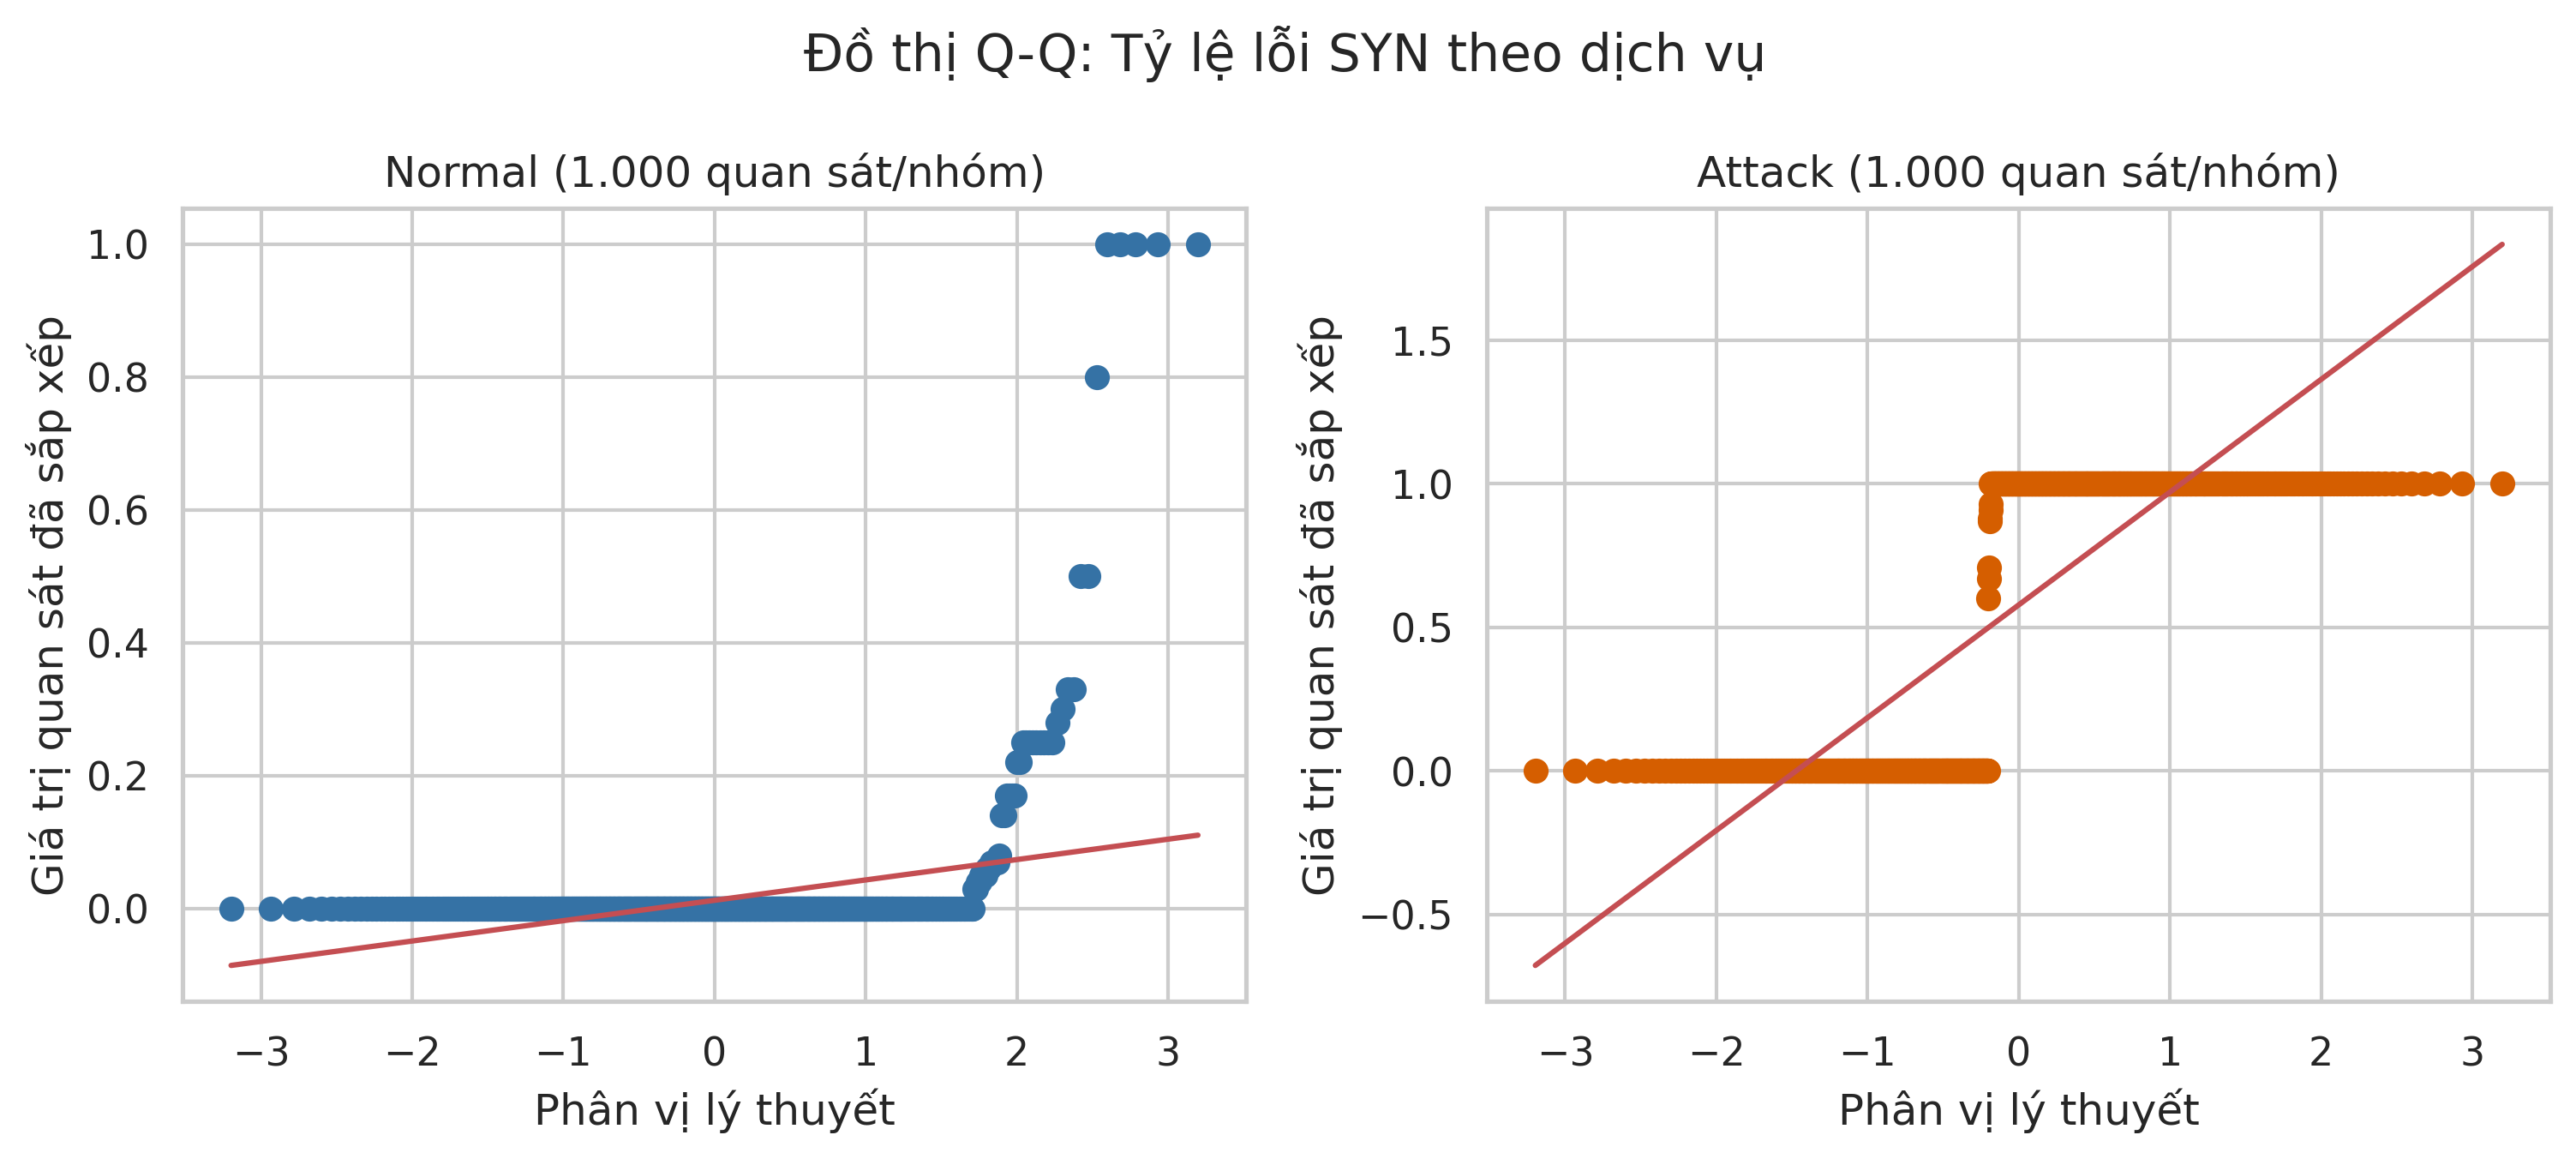
\includegraphics[width=0.97\linewidth]{srv_serror_rate/04_qq_plot.png}
\caption{Q--Q plot của \texttt{srv\_serror\_rate}. Các dải ngang tại 0 và 1 phản ánh
khối lượng xác suất tại hai biên; mỗi panel dùng tối đa 1.000 quan sát.}
\label{fig:two-sample-qq-serror}
\end{figure}

Hình~\ref{fig:two-sample-qq-serror} không tạo thành đám mây gần đường thẳng. Ở Normal,
phần lớn điểm nằm trên dải $y=0$, sau đó tăng đột ngột ở đuôi phải; skewness đạt 9,169.
Ở Attack, hai dải dày tại 0 và 1 tạo dạng gần nhị điểm, phù hợp với tỷ lệ bằng 0 là
40,486\% và bằng 1 là 58,920\%. Hai hình dạng khác nhau rõ và đều không phù hợp với
phân phối chuẩn của quan sát gốc.

\begin{figure}[H]
\centering
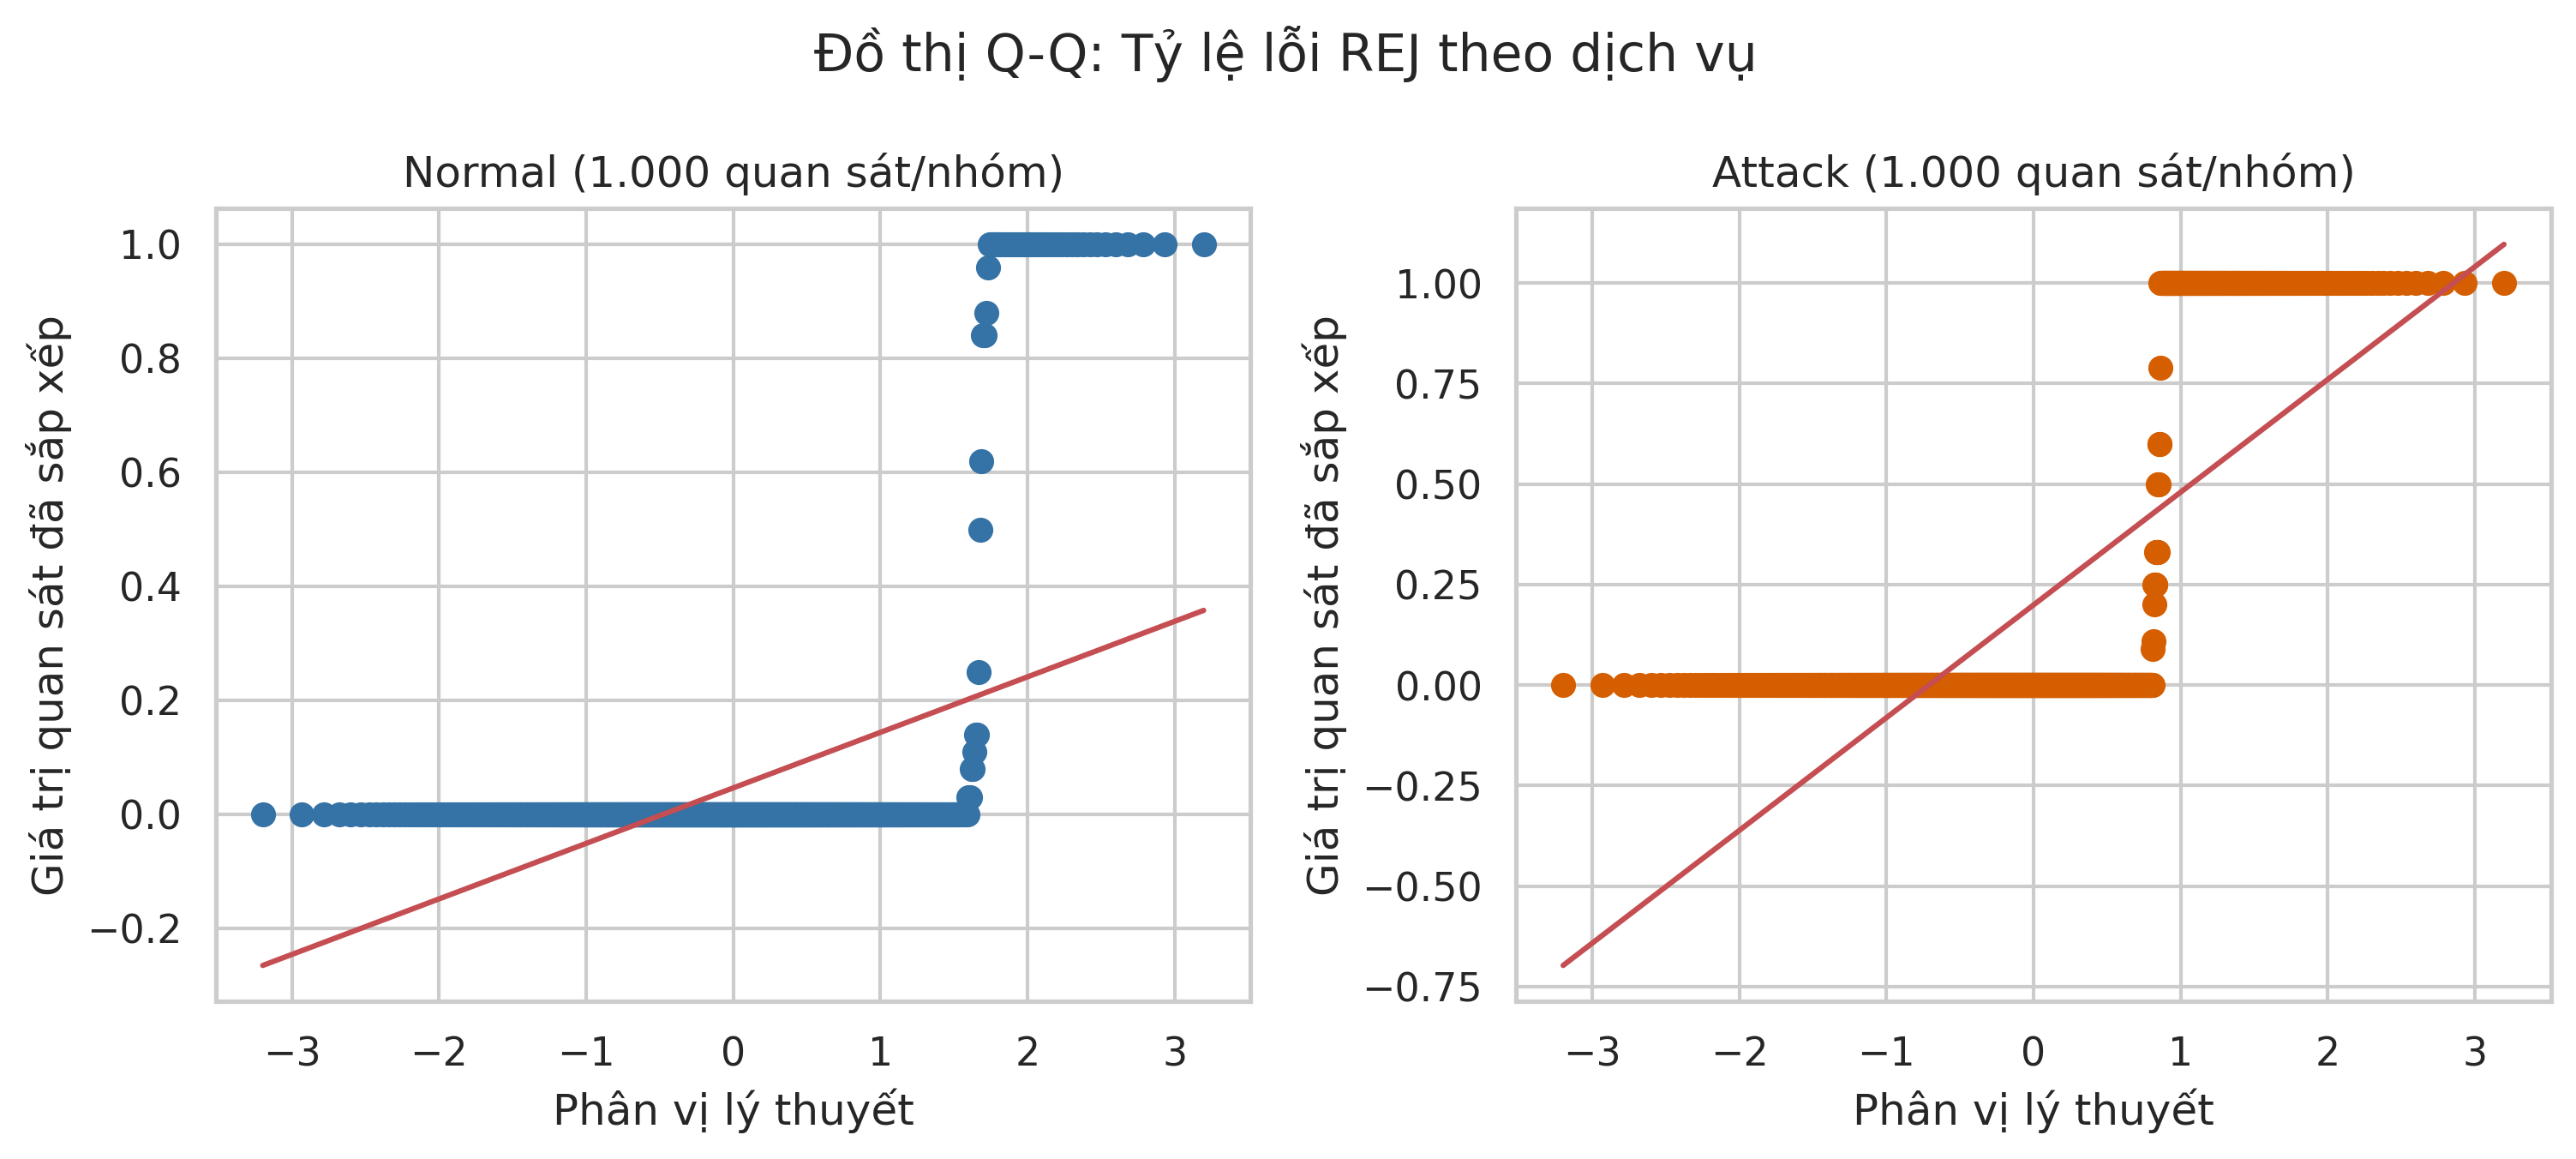
\includegraphics[width=0.97\linewidth]{srv_rerror_rate/04_qq_plot.png}
\caption{Q--Q plot của \texttt{srv\_rerror\_rate}. Các bậc và dải ngang xuất hiện do
biến tỷ lệ rời rạc, tập trung tại 0 và 1.}
\label{fig:two-sample-qq-rerror}
\end{figure}

Với \texttt{srv\_rerror\_rate}, Hình~\ref{fig:two-sample-qq-rerror} cũng có dải dài
tại 0, nhưng phần giá trị dương của Normal cong mạnh và nhảy lên dải 1 ở đuôi phải
(skewness 4,426). Attack có nhiều bậc trung gian hơn trước khi đạt 1 và vẫn lệch phải
(skewness 1,434). Đây không phải bản sao hình dạng RQ1: ở RQ2, trung vị và Q3 đều bằng
0 trong cả hai nhóm, cho thấy khối tại 0 chi phối mạnh hơn phần trung tâm.

\begin{figure}[H]
\centering
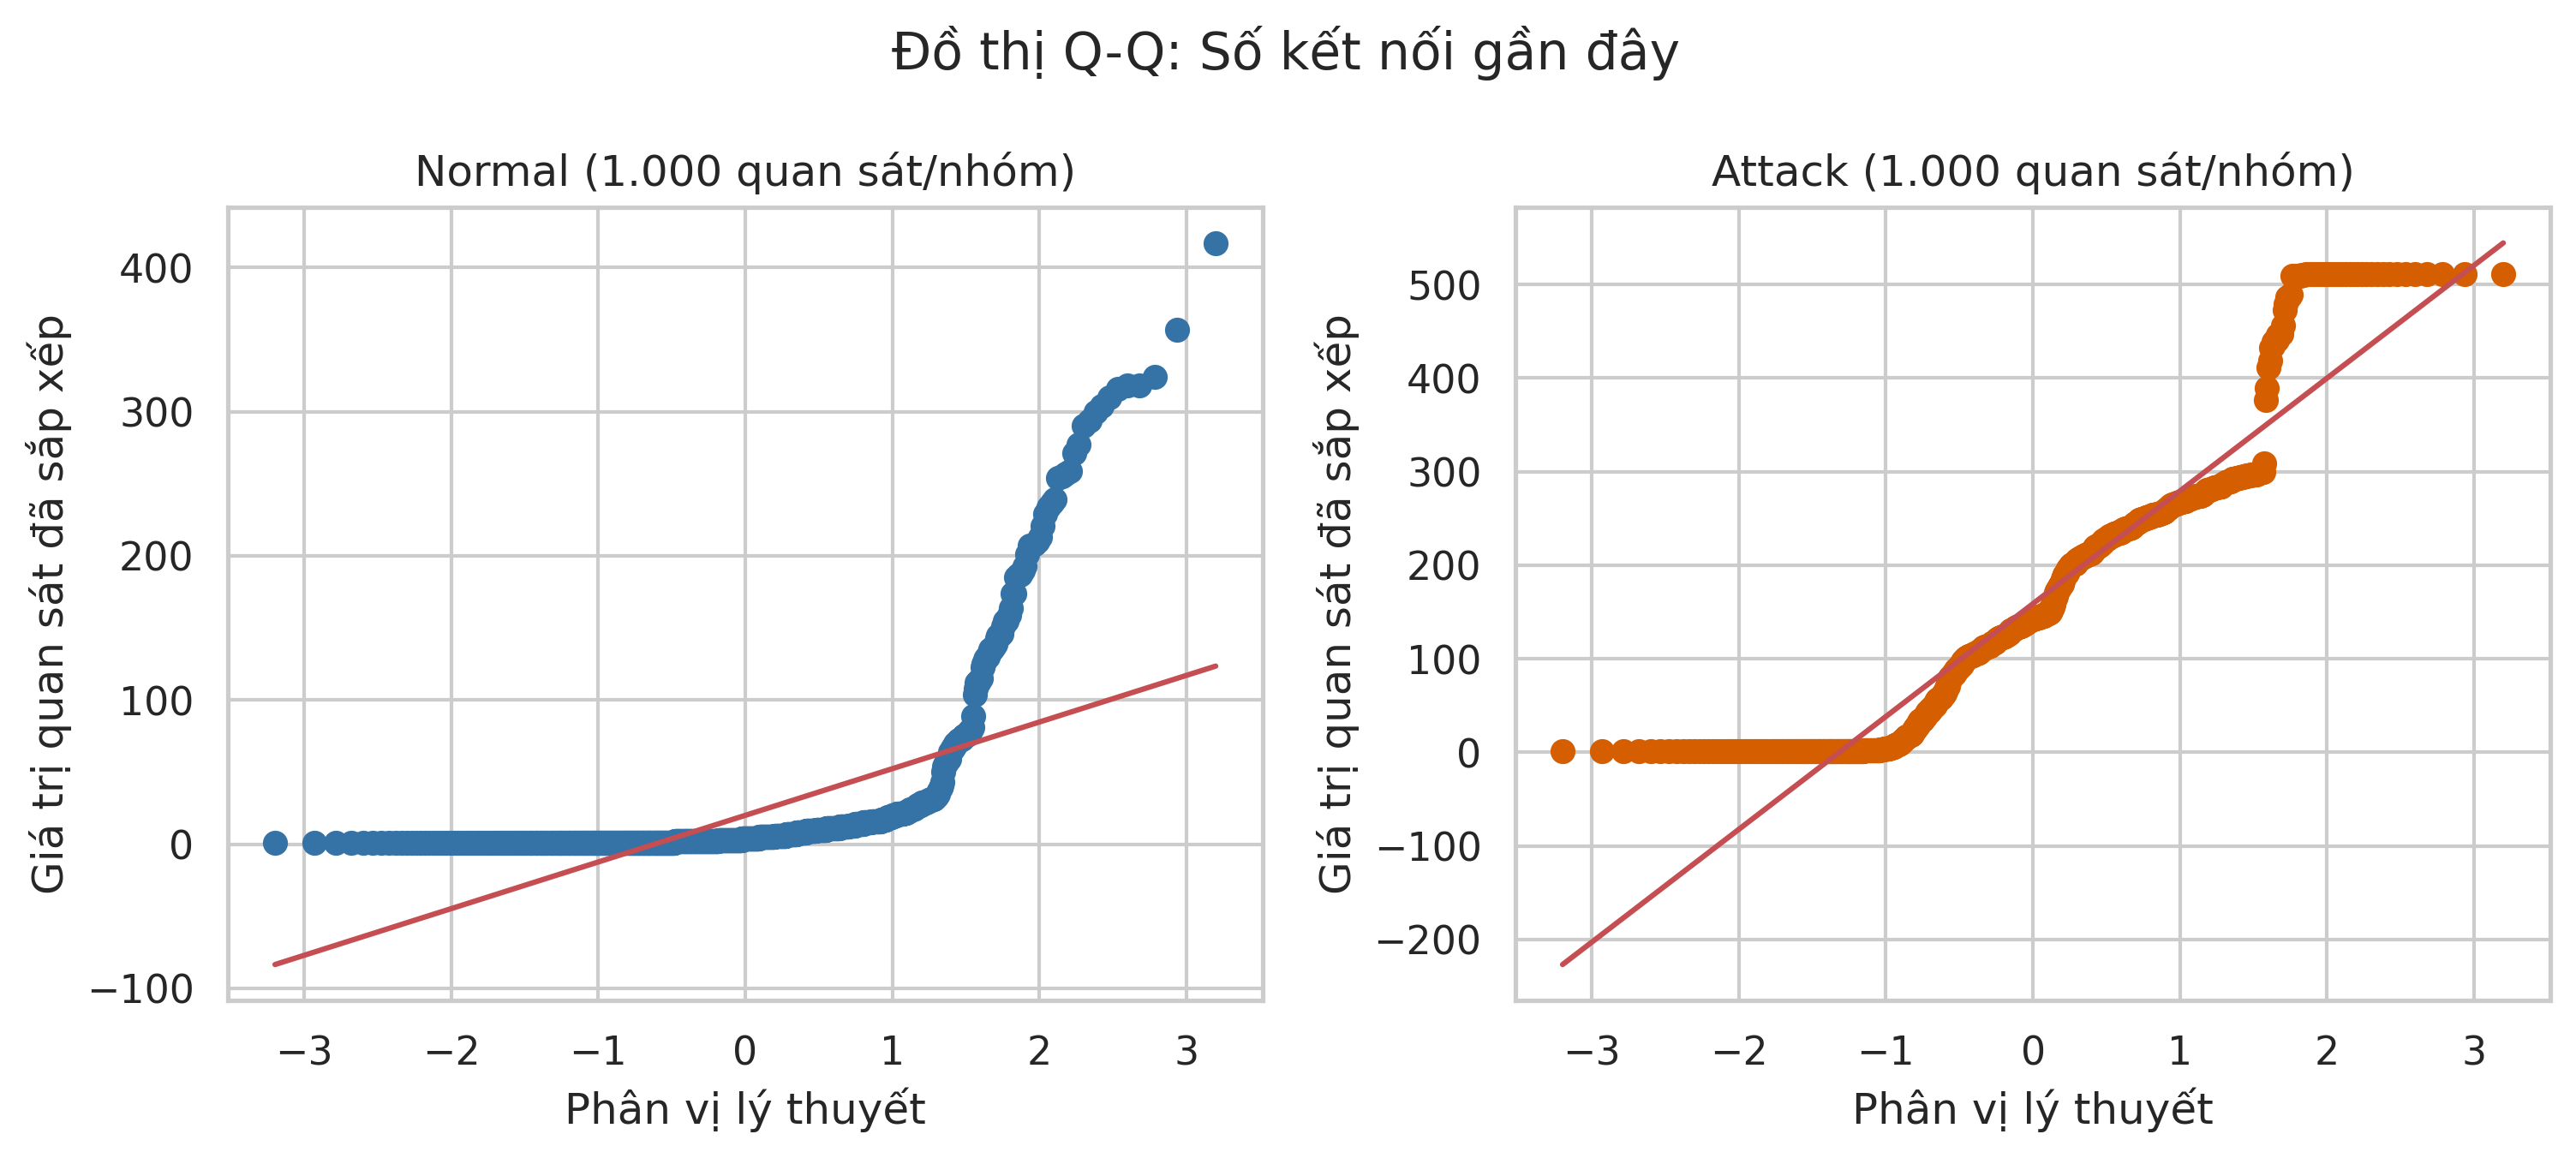
\includegraphics[width=0.97\linewidth]{count/04_qq_plot.png}
\caption{Q--Q plot của \texttt{count}. Normal có đuôi phải dài; Attack có dạng bậc
và trần tại 511, thể hiện tính rời rạc và bị chặn của biến đếm.}
\label{fig:two-sample-qq-count}
\end{figure}

Hình~\ref{fig:two-sample-qq-count} cho thấy Normal cong lên rất mạnh ở nửa phải và có
đuôi tới trên 400 trong mẫu vẽ, phù hợp skewness 3,878. Attack gần tuyến tính hơn ở
phần giữa nhưng lệch khỏi đường tham chiếu ở cả hai đuôi, có các bậc và dải ngang tại
511; skewness vẫn là 0,747. Q--Q plot vì vậy bác bỏ mô tả chuẩn đơn giản cho dữ liệu
gốc, đồng thời cho thấy dạng sai lệch của hai nhóm không giống nhau.

Q--Q plot chỉ là chẩn đoán trực quan. Cỡ mẫu lớn hỗ trợ xấp xỉ của trung bình mẫu,
nhưng không xóa khối biên, tính rời rạc hay phụ thuộc tiềm ẩn. Bảng
\ref{tab:two-sample-assumptions} bổ sung Brown--Forsythe và tỷ số phương sai; tất cả
đều cho thấy Student t-test phương sai gộp không thích hợp.

\begin{table}[H]
\centering
\caption{Chẩn đoán phương sai và hình dạng phân phối}
\label{tab:two-sample-assumptions}
\small
\setlength{\tabcolsep}{4pt}
\begin{tabularx}{\textwidth}{lrrrX}
\toprule
Đặc trưng & Brown--Forsythe & p-value & Tỷ số phương sai & Chẩn đoán trọng tâm \\
\midrule
\texttt{srv\_serror\_rate} & 42.179,95 & $<10^{-300}$ & 32,175 & Bị chặn; dồn mạnh tại 0 và 1. \\
\texttt{srv\_rerror\_rate} & 8.651,41 & $<10^{-300}$ & 3,999 & Q1=Q3=0; lệch phải và nhiều giá trị trùng. \\
\texttt{count} & 46.458,65 & $<10^{-300}$ & 5,296 & Biến đếm; Normal đuôi phải dài, hai nhóm cùng trần 511. \\
\bottomrule
\end{tabularx}
\end{table}

\begin{lstlisting}[
  caption={Lấy mẫu cố định chỉ để vẽ Q--Q plot (rút gọn từ mã thực tế).},
  label={lst:qq-code}]
for ax, group in zip(axes, GROUP_ORDER):
    values = plot_df.loc[
        plot_df["group"].eq(group), feature
    ].to_numpy(float)
    if len(values) > 1000:
        values = rng.choice(values, 1000, replace=False)
    stats.probplot(values, dist="norm", plot=ax)
\end{lstlisting}

\subsection{Kết quả kiểm định tỷ lệ lỗi SYN}
\label{subsec:two-sample-rq1}

RQ1 xem xét \texttt{srv\_serror\_rate}. Bằng chứng mô tả cho thấy Normal có trung
bình 0,01208 (KTC trung bình nhóm 95\%: 0,01143--0,01274), còn Attack là 0,59307
(0,58910--0,59704). Phương sai Attack lớn gấp 32,175 lần Normal và Q--Q plot có khối
biên rõ, nên Welch được giữ làm kiểm định chính thay vì Student t-test phương sai gộp.

\begin{table}[H]
\centering
\caption{Kết quả Welch cho RQ1 -- \texttt{srv\_serror\_rate}}
\label{tab:two-sample-rq1}
\small
\begin{tabular}{rrrrrrr}
\toprule
$\widehat\Delta$ & SE & $t$ & $\nu$ & p Holm & KTC 95\% của $\Delta$ & Hedges $g$ \\
\midrule
$-0{,}58099$ & 0,002052 & $-283{,}157$ & 61.805,40 & $<10^{-300}$ & $[-0{,}58501;-0{,}57697]$ & $-1{,}7070$ \\
\bottomrule
\end{tabular}
\end{table}

Khoảng tin cậy hoàn toàn âm và p-value Holm nhỏ hơn $10^{-300}$, do đó bác bỏ
$H_0$. Theo chiều định nghĩa Normal trừ Attack, kết quả tương ứng Attack cao hơn khoảng
0,581 đơn vị tỷ lệ. Hedges $g=-1{,}7070$ (KTC xấp xỉ
$[-1{,}7199;-1{,}6940]$) cho thấy chênh lệch chuẩn hóa đáng kể trong mẫu. Mann--Whitney
và Yuen--Welch 20\% đều cho $p<10^{-300}$, củng cố độ bền của kết luận về khác biệt,
nhưng không biến Welch thành mô hình hoàn chỉnh cho biến tỷ lệ dồn biên. Đặc trưng phản
ánh lỗi bắt tay TCP theo dịch vụ, không chứng minh lỗi SYN là nguyên nhân của tấn công.

\subsection{Kết quả kiểm định tỷ lệ lỗi REJ}
\label{subsec:two-sample-rq2}

RQ2 phân tích \texttt{srv\_rerror\_rate}. Normal có trung bình 0,04463, Attack là
0,20911; dù vậy, trung vị và Q3 của cả hai nhóm đều bằng 0. Sự kết hợp giữa khối tại 0
và phương sai Attack gấp 3,999 lần Normal là lý do không diễn giải chênh lệch trung
bình như khác biệt đồng đều ở mọi kết nối.

\begin{table}[H]
\centering
\caption{Kết quả Welch cho RQ2 -- \texttt{srv\_rerror\_rate}}
\label{tab:two-sample-rq2}
\small
\begin{tabular}{rrrrrrr}
\toprule
$\widehat\Delta$ & SE & $t$ & $\nu$ & p Holm & KTC 95\% của $\Delta$ & Hedges $g$ \\
\midrule
$-0{,}16448$ & 0,001843 & $-89{,}230$ & 83.489,74 & $<10^{-300}$ & $[-0{,}16810;-0{,}16087]$ & $-0{,}5254$ \\
\bottomrule
\end{tabular}
\end{table}

Bác bỏ $H_0$ sau hiệu chỉnh Holm. Attack cao hơn Normal khoảng 0,1645 đơn vị tỷ lệ;
Hedges $g=-0{,}5254$ (KTC xấp xỉ $[-0{,}5366;-0{,}5141]$) nhỏ hơn về trị tuyệt đối
so với RQ1. Mann--Whitney cho $p<10^{-300}$; Yuen--Welch cho
$p=4{,}905\times10^{-8}$ với chênh lệch trung bình cắt ngọn chỉ $-0{,}01519$. Sự
giảm mạnh sau cắt ngọn cho thấy chênh lệch trung bình gốc chịu ảnh hưởng đáng kể của
khối giá trị lớn, dù bằng chứng về khác biệt vẫn còn. Đây là tín hiệu về lỗi REJ theo
dịch vụ, không phải bằng chứng rằng một ngưỡng đơn biến đủ nhận diện Attack.

\subsection{Kết quả kiểm định số lượng kết nối gần đây}
\label{subsec:two-sample-rq3}

RQ3 xét \texttt{count}. Normal có trung bình 22,518 và trung vị 4, trong khi Attack
có trung bình 154,850 và trung vị 138. Chênh lệch của cả trung bình lẫn trung vị cùng
hướng, nhưng độ lệch phải, ngoại lệ và trần 511 cho thấy phân bố không chuẩn.

\begin{table}[H]
\centering
\caption{Kết quả Welch cho RQ3 -- \texttt{count}}
\label{tab:two-sample-rq3}
\small
\begin{tabular}{rrrrrrr}
\toprule
$\widehat\Delta$ & SE & $t$ & $\nu$ & p Holm & KTC 95\% của $\Delta$ & Hedges $g$ \\
\midrule
$-132{,}332$ & 0,5541 & $-238{,}828$ & 77.661,21 & $<10^{-300}$ & $[-133{,}418;-131{,}246]$ & $-1{,}4143$ \\
\bottomrule
\end{tabular}
\end{table}

Khoảng tin cậy cho thấy Attack cao hơn Normal khoảng 131,246--133,418 kết nối trung
bình trong định nghĩa cửa sổ của NSL-KDD. Bác bỏ $H_0$ sau Holm; Hedges
$g=-1{,}4143$ (KTC xấp xỉ $[-1{,}4266;-1{,}4019]$). Mann--Whitney và Yuen--Welch
đều có $p<10^{-300}$; chênh lệch trung bình cắt ngọn là $-140{,}988$. Kết quả phù hợp
với việc nhiều hành vi Attack tạo kết nối tập trung trong thời gian ngắn, nhưng nhóm
Attack là hỗn hợp bốn họ và hai miền giá trị vẫn chồng lấp; không thể suy ra mọi dạng
tấn công đều có \texttt{count} cao.

Mã tính Welch, bậc tự do và khoảng tin cậy dùng cùng một sai số chuẩn được rút gọn từ
module tại Đoạn mã~\ref{lst:welch-code}; công thức và chiều chênh lệch không thay đổi.
\begin{minipage}{\textwidth}
\begin{lstlisting}[
  caption={Hàm Welch và KTC chênh lệch trung bình (rút gọn từ mã thực tế).},
  label={lst:welch-code}]
def welch_test(x, y, alpha=ALPHA):
    n1, n2 = x.size, y.size
    m1, m2 = np.mean(x), np.mean(y)
    s1, s2 = np.var(x, ddof=1), np.var(y, ddof=1)
    v1, v2 = s1 / n1, s2 / n2
    se = np.sqrt(v1 + v2)
    diff = m1 - m2
    df = (v1 + v2) ** 2 / (
        v1**2 / (n1 - 1) + v2**2 / (n2 - 1)
    )
    t_stat = diff / se
    p_value = 2 * stats.t.sf(abs(t_stat), df)
    critical = stats.t.ppf(1 - alpha / 2, df)
    ci95 = (diff - critical * se, diff + critical * se)
    return diff, se, t_stat, df, p_value, ci95
\end{lstlisting}
\end{minipage}

\subsection{So sánh tổng hợp ba kiểm định}
\label{subsec:two-sample-summary}

\begin{table}[H]
\centering
\caption{Tổng hợp ba kiểm định Welch hai mẫu độc lập}
\label{tab:two-sample-summary}
\scriptsize
\setlength{\tabcolsep}{2.5pt}
\resizebox{\textwidth}{!}{%
\begin{tabular}{lrrrrrrrrl}
\toprule
Biến & TB N & TB A & $\widehat\Delta$ & $t$ & $\nu$ & p thô & p Holm & KTC 95\% & $g$ / Quyết định \\
\midrule
\texttt{srv\_serror\_rate} & 0,01208 & 0,59307 & $-0,58099$ & $-283,157$ & 61.805,40 & $<10^{-300}$ & $<10^{-300}$ & $[-0,58501;-0,57697]$ & $-1,7070$ / Bác bỏ $H_0$ \\
\texttt{srv\_rerror\_rate} & 0,04463 & 0,20911 & $-0,16448$ & $-89,230$ & 83.489,74 & $<10^{-300}$ & $<10^{-300}$ & $[-0,16810;-0,16087]$ & $-0,5254$ / Bác bỏ $H_0$ \\
\texttt{count} & 22,518 & 154,850 & $-132,332$ & $-238,828$ & 77.661,21 & $<10^{-300}$ & $<10^{-300}$ & $[-133,418;-131,246]$ & $-1,4143$ / Bác bỏ $H_0$ \\
\bottomrule
\end{tabular}}
\par\smallskip
\footnotesize TB N/A: trung bình Normal/Attack; $\widehat\Delta=$ Normal $-$ Attack.
Hedges $g$ dùng SD gộp và được xem là effect size mô tả khi phương sai khác nhau.
\end{table}

\begin{figure}[H]
\centering
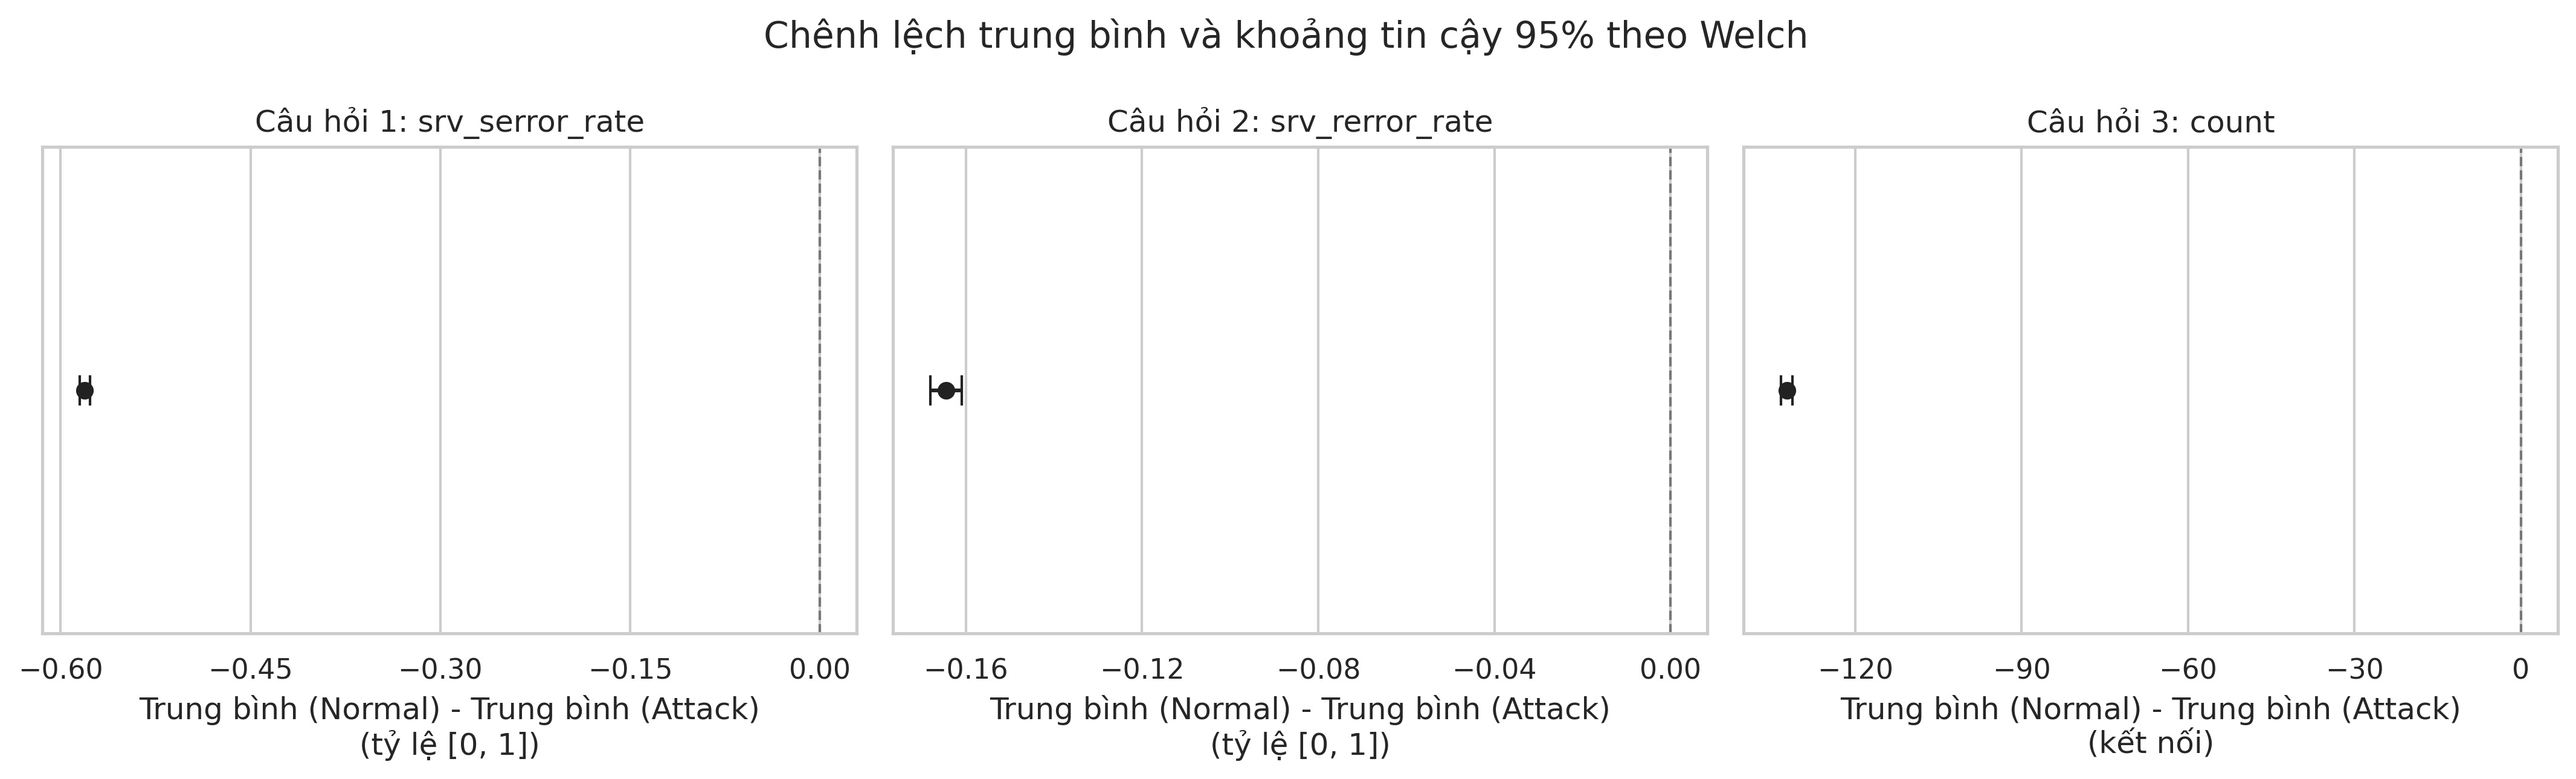
\includegraphics[width=0.98\linewidth]{comparison/mean_difference_forest.png}
\caption{Chênh lệch trung bình Normal $-$ Attack và KTC 95\% theo Welch. Ba panel
dùng trục riêng vì đặc trưng có đơn vị khác nhau; đường đứt đoạn tại 0 là mốc không
chênh lệch.}
\label{fig:two-sample-mean-difference}
\end{figure}

\begin{figure}[H]
\centering
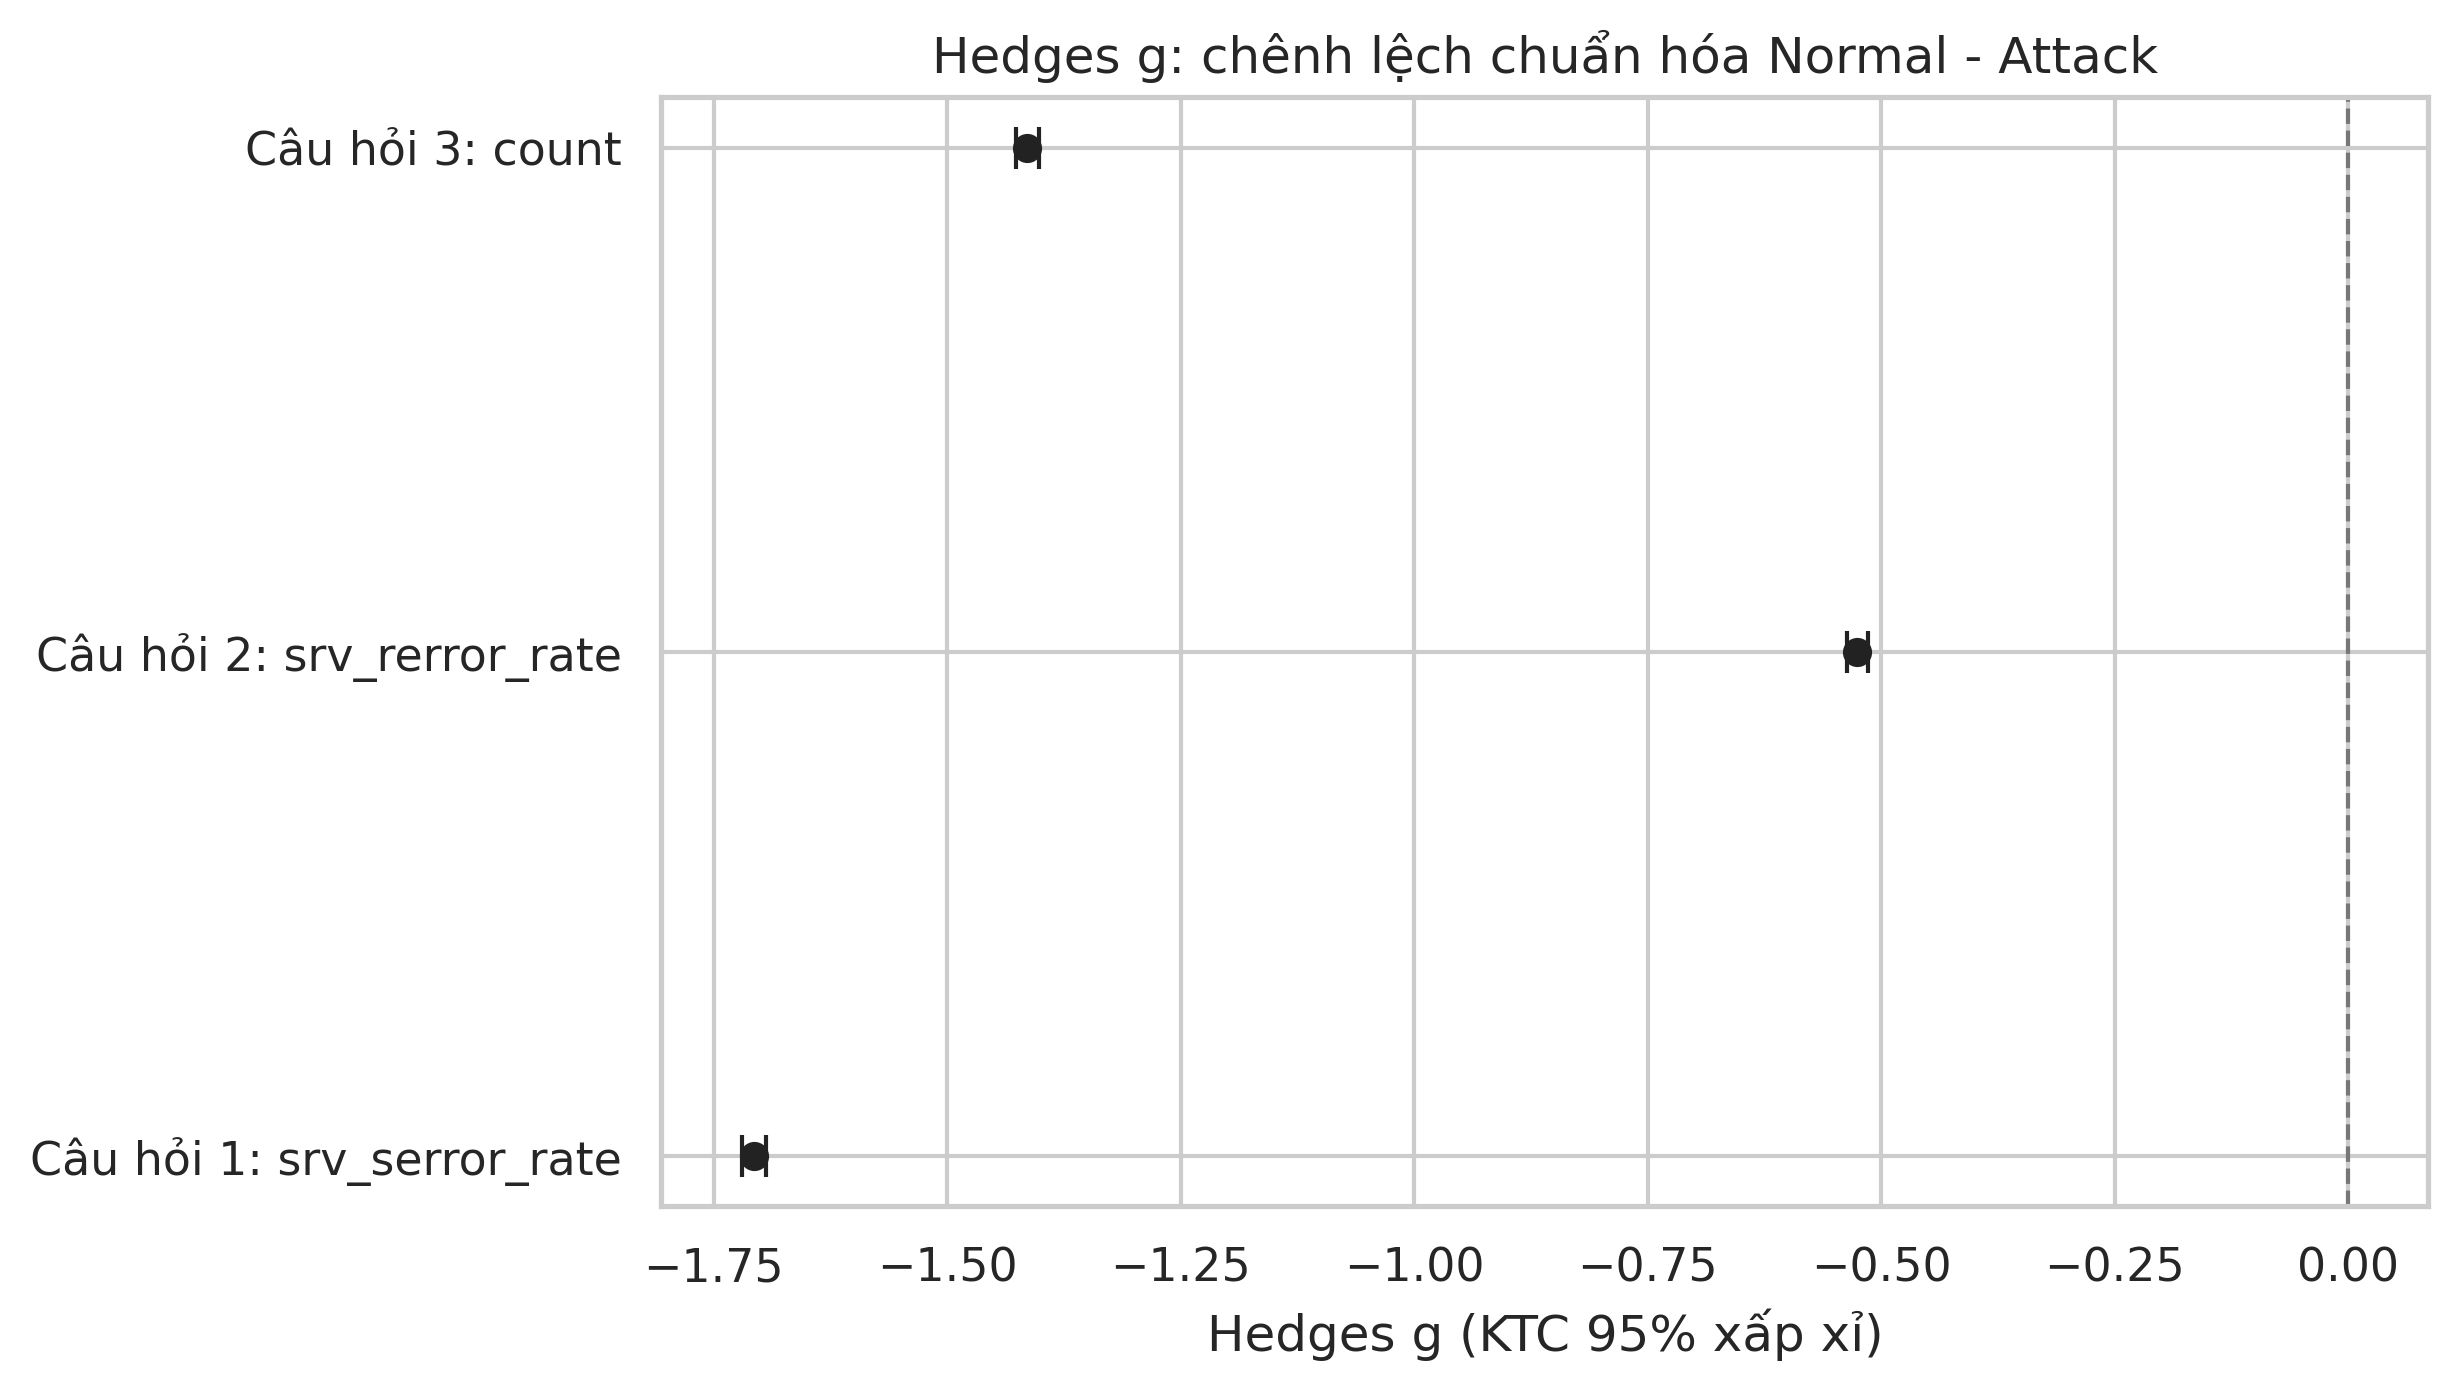
\includegraphics[width=0.80\linewidth]{comparison/effect_size_forest.png}
\caption{Hedges $g$ và KTC 95\% xấp xỉ cho ba RQ. Trị tuyệt đối lớn không được diễn
giải là năng lực dự đoán ngoài mẫu.}
\label{fig:two-sample-effect-size}
\end{figure}

Cả ba giả thuyết bị bác bỏ sau Holm, nhưng mức độ và hình dạng khác biệt không giống
nhau. RQ1 và RQ3 có chênh lệch chuẩn hóa lớn trong mẫu; RQ2 nhỏ hơn và nhạy hơn với
cắt ngọn. Các biến tỷ lệ gây khó khăn vì khối biên, còn \texttt{count} gây khó khăn
do tính rời rạc, lệch phải và trần dữ liệu. Do cỡ mẫu rất lớn, p-value cực nhỏ phải
được đọc cùng khoảng tin cậy, effect size và phân bố chồng lấp.

Kết quả bổ sung cho Pearson: hệ số Pearson hiện có giữa
\path{srv_serror_rate} và \path{dst_host_srv_serror_rate} là 0,9863; giữa
\path{srv_rerror_rate} và \path{dst_host_srv_rerror_rate} là 0,9702.
Các hệ số này cho biết tính dư thừa tuyến tính giữa đặc trưng, còn Welch cho biết
chênh lệch trung bình theo nhãn. ANOVA năm nhóm đối với \texttt{count} trả lời câu hỏi
khác: nó giữ riêng DoS, Probe, R2L, U2R, trong khi phân tích này gộp chúng thành Attack.
Hai phân tích dùng cùng bản ghi nên không độc lập về thông tin.

\FloatBarrier



\end{document}

